\begin{spacing}{1}
    \chapter*{Abstract [L]}
\end{spacing}
\begin{wrapfigure}{r}{0.3\textwidth}
    \begin{center}
      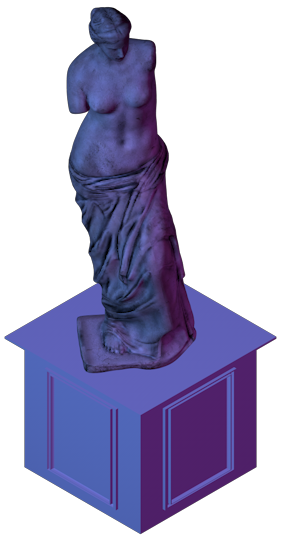
\includegraphics[width=0.2\textwidth]{pics/statue.png}
    \end{center}
\end{wrapfigure}
\setauthor{Litzlbauer Lorenz}
3D Portfolio Gallery is a web application that was developed by Lorenz Litzlbauer and Fabian Maar as part of their diploma thesis. 3D Portfolio Gallery aims to enable designers to share their design portfolio with the world in an innovative way, all in a virtual three-dimensional space. The designers can use the 3D Portfolio Gallery to create a three-dimensional portfolio from their own media (film, photo or 3D data).

3D Portfolio Gallery is offered as an SPA on the web and is accessible via a web link. 3D Portfolio Gallery offers a simple configuration process for this by selecting a gallery from several predefined floor plans. In a further step, the exhibits are placed either automatically or manually and provided with additional information.

Those interested can move freely through the three-dimensional
web exhibition and view the exhibits with different types of interaction.

The following frameworks are used for implementation in the frontend: Angular for the SPA (single-page application) and ThreeJs for the 3D display. JWT (JsonWebToken) is used in the frontend access control and user identification in the browser.
\newpage
\begin{spacing}{1}
    \chapter*{Zusammenfassung [L]}
\end{spacing}
\begin{wrapfigure}{r}{0.3\textwidth}
    \begin{center}
      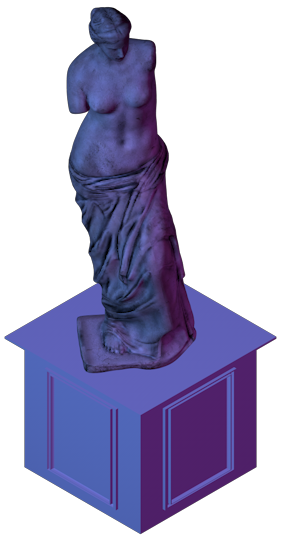
\includegraphics[width=0.2\textwidth]{pics/statue.png}
    \end{center}
\end{wrapfigure}
\setauthor{Litzlbauer Lorenz}
3D Portfolio Gallery ist eine Webapplikation, Lorenz Litzlbauer und Fabian Maar im Rahmen der Diplomarbeit entwickelt wurde. 3D Portfolio Gallery will Designer*innen ermöglichen, ihr Design-Portfolio auf eine innovative Art und Weise mit der Welt zu teilen und das alles in einem virtuellen dreidimensionalen Raum. Die Designer*innen können mithilfe von 3D Portfolio Gallery aus eigenen Medien (Film, Foto oder 3D-Daten) ein dreidimensionales Portfolio erstellen.

3D Portfolio Gallery wird als eine SPA im Web angeboten und ist über einen Web-Link erreichbar. 3D Portfolio Gallery bietet dafür einen einfachen Konfigurationsprozess, indem aus mehreren vordefinierten Grundrissen eine Gallery ausgewählt wird. In einem weiteren Schritt werden die Ausstellungsstücke entweder automatisch oder manuell platziert und mit Zusatzinformationen versehen.

Interessierte können sich in der dreidimensionalen Webausstellung frei bewegen und die
Ausstellungsstücke mit verschiedenen Interaktionsarten anschauen.

Für die Umsetzung im Frontend werden folgende Frameworks verwendet: Angular für die SPA (Single-Page-Applikation) und ThreeJs für die 3D-Darstellung. In der Frontend-Zugriffkontrolle und -Useridentifikation im Browser wird JWT (JsonWebToken) verwendet.